\documentclass{standalone}
\usepackage{tikz}
\usetikzlibrary{patterns, positioning}


\begin{document}
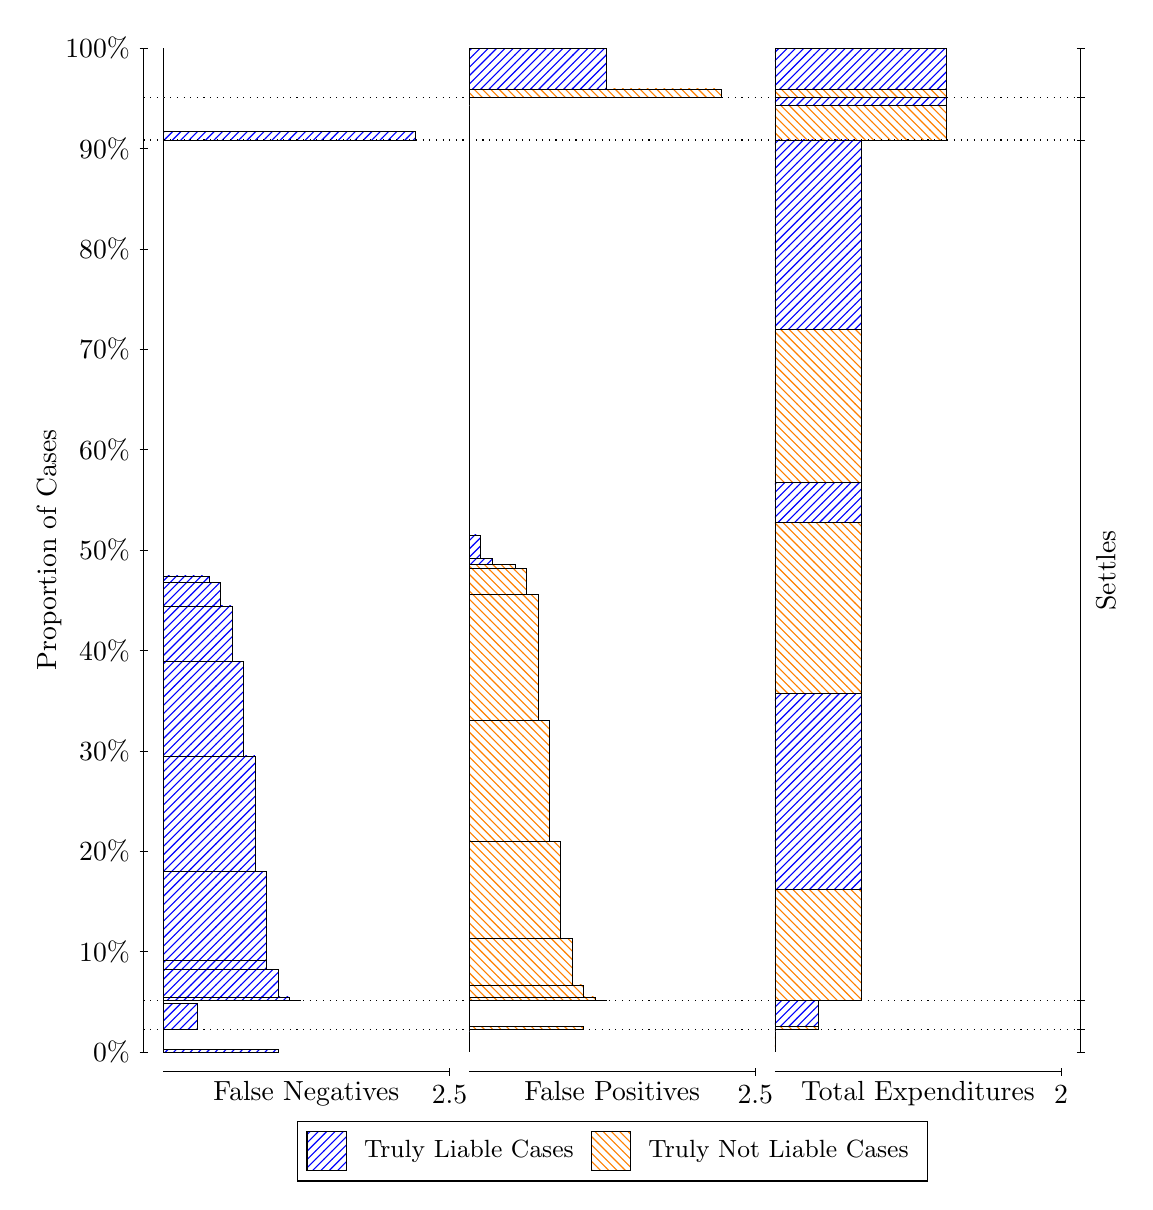
\begin{tikzpicture}
\draw[black, very thin] (1.5,1.75) -- (1.5,14.5);
\node[rotate=90, text=black, anchor=center] at (0.3, 8.125) {Proportion of Cases};
\draw[black, very thin] (1.45,1.75) -- (1.55,1.75);
\node[text=black, anchor=east] at (1.45, 1.75) {0\%};
\draw[black, very thin] (1.45,3.025) -- (1.55,3.025);
\node[text=black, anchor=east] at (1.45, 3.025) {10\%};
\draw[black, very thin] (1.45,4.3) -- (1.55,4.3);
\node[text=black, anchor=east] at (1.45, 4.3) {20\%};
\draw[black, very thin] (1.45,5.575) -- (1.55,5.575);
\node[text=black, anchor=east] at (1.45, 5.575) {30\%};
\draw[black, very thin] (1.45,6.85) -- (1.55,6.85);
\node[text=black, anchor=east] at (1.45, 6.85) {40\%};
\draw[black, very thin] (1.45,8.125) -- (1.55,8.125);
\node[text=black, anchor=east] at (1.45, 8.125) {50\%};
\draw[black, very thin] (1.45,9.4) -- (1.55,9.4);
\node[text=black, anchor=east] at (1.45, 9.4) {60\%};
\draw[black, very thin] (1.45,10.675) -- (1.55,10.675);
\node[text=black, anchor=east] at (1.45, 10.675) {70\%};
\draw[black, very thin] (1.45,11.95) -- (1.55,11.95);
\node[text=black, anchor=east] at (1.45, 11.95) {80\%};
\draw[black, very thin] (1.45,13.225) -- (1.55,13.225);
\node[text=black, anchor=east] at (1.45, 13.225) {90\%};
\draw[black, very thin] (1.45,14.5) -- (1.55,14.5);
\node[text=black, anchor=east] at (1.45, 14.5) {100\%};

\draw[black, very thin] (13.4,1.75) -- (13.4,14.5);
\draw[black, very thin] (13.35,1.75) -- (13.45,1.75);
\node[anchor=west] at (13.35, 1.75) {};
\draw[black, very thin] (13.35,2.0381) -- (13.45,2.0381);
\node[anchor=west] at (13.35, 2.0381) {};
\draw[black, very thin] (13.35,2.4008) -- (13.45,2.4008);
\node[anchor=west] at (13.35, 2.4008) {};
\draw[black, very thin] (13.35,13.332) -- (13.45,13.332);
\node[anchor=west] at (13.35, 13.332) {};
\draw[black, very thin] (13.35,13.874) -- (13.45,13.874);
\node[anchor=west] at (13.35, 13.874) {};
\draw[black, very thin] (13.35,14.5) -- (13.45,14.5);
\node[anchor=west] at (13.35, 14.5) {};

\draw[black, very thin, pattern color=blue, pattern=north east lines] (1.75,1.75) rectangle (3.2033,1.7803);
\draw[black, very thin, pattern color=orange, pattern=north west lines] (1.75,1.7803) rectangle (1.75,2.0381);
\draw[black, very thin, pattern color=blue, pattern=north east lines] (1.75,2.0381) rectangle (2.186,2.3628);
\draw[black, very thin, pattern color=orange, pattern=north west lines] (1.75,2.3628) rectangle (1.75,2.4008);
\draw[black, very thin, pattern color=blue, pattern=north east lines] (1.75,2.4008) rectangle (3.494,2.4052);
\draw[black, very thin, pattern color=blue, pattern=north east lines] (1.75,2.4052) rectangle (3.3487,2.4505);
\draw[black, very thin, pattern color=blue, pattern=north east lines] (1.75,2.4505) rectangle (3.2033,2.8034);
\draw[black, very thin, pattern color=blue, pattern=north east lines] (1.75,2.8034) rectangle (3.058,2.9088);
\draw[black, very thin, pattern color=blue, pattern=north east lines] (1.75,2.9088) rectangle (3.058,4.0393);
\draw[black, very thin, pattern color=blue, pattern=north east lines] (1.75,4.0393) rectangle (2.9127,5.5115);
\draw[black, very thin, pattern color=blue, pattern=north east lines] (1.75,5.5115) rectangle (2.7673,6.709);
\draw[black, very thin, pattern color=blue, pattern=north east lines] (1.75,6.709) rectangle (2.622,7.4156);
\draw[black, very thin, pattern color=blue, pattern=north east lines] (1.75,7.4156) rectangle (2.4767,7.718);
\draw[black, very thin, pattern color=blue, pattern=north east lines] (1.75,7.718) rectangle (2.3313,7.7957);
\draw[black, very thin, pattern color=orange, pattern=north west lines] (1.75,7.7957) rectangle (1.75,13.332);
\draw[black, very thin, pattern color=blue, pattern=north east lines] (1.75,13.332) rectangle (4.9473,13.438);
\draw[black, very thin, pattern color=orange, pattern=north west lines] (1.75,13.438) rectangle (1.75,13.874);
\draw[black, very thin, pattern color=orange, pattern=north west lines] (1.75,13.874) rectangle (1.75,13.98);
\draw[black, very thin, pattern color=blue, pattern=north east lines] (1.75,13.98) rectangle (1.75,14.5);
\draw[black, very thin, pattern color=orange, pattern=north west lines] (5.6333,1.75) rectangle (5.6333,2.0078);
\draw[black, very thin, pattern color=blue, pattern=north east lines] (5.6333,2.0078) rectangle (5.6333,2.0381);
\draw[black, very thin, pattern color=orange, pattern=north west lines] (5.6333,2.0381) rectangle (7.0867,2.0761);
\draw[black, very thin, pattern color=blue, pattern=north east lines] (5.6333,2.0761) rectangle (5.6333,2.4008);
\draw[black, very thin, pattern color=orange, pattern=north west lines] (5.6333,2.4008) rectangle (7.3773,2.4089);
\draw[black, very thin, pattern color=orange, pattern=north west lines] (5.6333,2.4089) rectangle (7.232,2.4499);
\draw[black, very thin, pattern color=orange, pattern=north west lines] (5.6333,2.4499) rectangle (7.0867,2.6023);
\draw[black, very thin, pattern color=orange, pattern=north west lines] (5.6333,2.6023) rectangle (6.9413,3.1971);
\draw[black, very thin, pattern color=orange, pattern=north west lines] (5.6333,3.1971) rectangle (6.796,4.4221);
\draw[black, very thin, pattern color=orange, pattern=north west lines] (5.6333,4.4221) rectangle (6.6507,5.9615);
\draw[black, very thin, pattern color=orange, pattern=north west lines] (5.6333,5.9615) rectangle (6.5053,7.5633);
\draw[black, very thin, pattern color=orange, pattern=north west lines] (5.6333,7.5633) rectangle (6.36,7.896);
\draw[black, very thin, pattern color=orange, pattern=north west lines] (5.6333,7.896) rectangle (6.2147,7.9375);
\draw[black, very thin, pattern color=blue, pattern=north east lines] (5.6333,7.9375) rectangle (5.924,8.0152);
\draw[black, very thin, pattern color=blue, pattern=north east lines] (5.6333,8.0152) rectangle (5.7787,8.3176);
\draw[black, very thin, pattern color=blue, pattern=north east lines] (5.6333,8.3176) rectangle (5.6333,13.332);
\draw[black, very thin, pattern color=orange, pattern=north west lines] (5.6333,13.332) rectangle (5.6333,13.769);
\draw[black, very thin, pattern color=blue, pattern=north east lines] (5.6333,13.769) rectangle (5.6333,13.874);
\draw[black, very thin, pattern color=orange, pattern=north west lines] (5.6333,13.874) rectangle (8.8307,13.98);
\draw[black, very thin, pattern color=blue, pattern=north east lines] (5.6333,13.98) rectangle (7.3773,14.5);
\draw[black, very thin, pattern color=orange, pattern=north west lines] (9.5167,1.75) rectangle (9.5167,2.0078);
\draw[black, very thin, pattern color=blue, pattern=north east lines] (9.5167,2.0078) rectangle (9.5167,2.0381);
\draw[black, very thin, pattern color=orange, pattern=north west lines] (9.5167,2.0381) rectangle (10.062,2.0761);
\draw[black, very thin, pattern color=blue, pattern=north east lines] (9.5167,2.0761) rectangle (10.062,2.4008);
\draw[black, very thin, pattern color=orange, pattern=north west lines] (9.5167,2.4008) rectangle (10.607,3.8192);
\draw[black, very thin, pattern color=blue, pattern=north east lines] (9.5167,3.8192) rectangle (10.607,6.3003);
\draw[black, very thin, pattern color=orange, pattern=north west lines] (9.5167,6.3003) rectangle (10.607,8.472);
\draw[black, very thin, pattern color=blue, pattern=north east lines] (9.5167,8.472) rectangle (10.607,8.9799);
\draw[black, very thin, pattern color=orange, pattern=north west lines] (9.5167,8.9799) rectangle (10.607,10.926);
\draw[black, very thin, pattern color=blue, pattern=north east lines] (9.5167,10.926) rectangle (10.607,13.332);
\draw[black, very thin, pattern color=orange, pattern=north west lines] (9.5167,13.332) rectangle (11.697,13.769);
\draw[black, very thin, pattern color=blue, pattern=north east lines] (9.5167,13.769) rectangle (11.697,13.874);
\draw[black, very thin, pattern color=orange, pattern=north west lines] (9.5167,13.874) rectangle (11.697,13.98);
\draw[black, very thin, pattern color=blue, pattern=north east lines] (9.5167,13.98) rectangle (11.697,14.5);
\draw[black, dotted] (1.5,2.0381) -- (13.4,2.0381);
\draw[black, dotted] (1.5,2.4008) -- (13.4,2.4008);
\draw[black, dotted] (1.5,13.332) -- (13.4,13.332);
\draw[black, dotted] (1.5,13.874) -- (13.4,13.874);
\draw[black, very thin] (1.75,1.5) -- (5.3833,1.5);
\node[text=black, anchor=north] at (3.5667, 1.5) {False Negatives};
\draw[black, very thin] (5.3833,1.45) -- (5.3833,1.55);
\node[text=black, anchor=north] at (5.3833, 1.45) {2.5};

\draw[black, very thin] (5.6333,1.5) -- (9.2667,1.5);
\node[text=black, anchor=north] at (7.45, 1.5) {False Positives};
\draw[black, very thin] (9.2667,1.45) -- (9.2667,1.55);
\node[text=black, anchor=north] at (9.2667, 1.45) {2.5};

\draw[black, very thin] (9.5167,1.5) -- (13.15,1.5);
\node[text=black, anchor=north] at (11.333, 1.5) {Total Expenditures};
\draw[black, very thin] (13.15,1.45) -- (13.15,1.55);
\node[text=black, anchor=north] at (13.15, 1.45) {2};



\node[text=black, centered, rotate=90] at (13.72, 7.8666) {Settles};



\draw (7.449999999999999,1.5) node[draw=none] (baseCoordinate) {};
\begin{scope}[align=center]
        \matrix[scale=0.5, draw=black, below=0.5cm of baseCoordinate, nodes={draw}, column sep=0.1cm]{
            \node[rectangle, draw, minimum width=0.5cm, minimum height=0.5cm, pattern color=blue, pattern=north east lines] {}; &
            \node[draw=none, font=\small, text=black] (B) {Truly Liable Cases}; &
            \node[rectangle, draw, minimum width=0.5cm, minimum height=0.5cm, pattern color=orange, pattern=north west lines] {}; &
            \node[draw=none, font=\small, text=black] (B) {Truly Not Liable Cases}; \\
            };
\end{scope}

\end{tikzpicture}
\end{document}